\chapter{Methodology}
\label{chapter:methodology}


\section{Work Plan}

In this section is presented the work plan for this thesis. In Figure \ref{fig:c3:gantt_chart} is displayed a Gantt chart which maps the timeline of each task in the development process. The purpose of this work plan is to ensure a systematic approach to the development and writing of this thesis. It reflects a thoughtful and comprehensive approach to tackling a complex and dynamic problem in cybersecurity. The work plan is divided into three main phases: \textit{Research}, \textit{Development} and \textit{Writing}, not being treated separately but rather as a continuous process. 

The plan spans over ten months, with each task carefully allocated to specific weeks within these months, enabling a clear roadmap for the thesis progression. The next steps are described in more detail:
\begin{itemize}
    \item \textbf{Research:} To finish this phase, it is necessary to complete the architecture planning and the models to be used;
    \item \textbf{Development:} In this phase, the development of the framework will be carried out, as well as the tests and validation of the results. This involves two main tasks: Phishing detection and sentiment analysis module development. Testing the model with real data and identifying possible limitations are addressed in this phase;
    \item \textbf{Writing:} The writing of the thesis will be done in parallel with the development of the framework so that the writing of the thesis is not left to the end. This includes the writing of the proposal chapter as well as the completion of the rest of the thesis. 
\end{itemize}

\begin{figure}[H]
    \begin{center}
        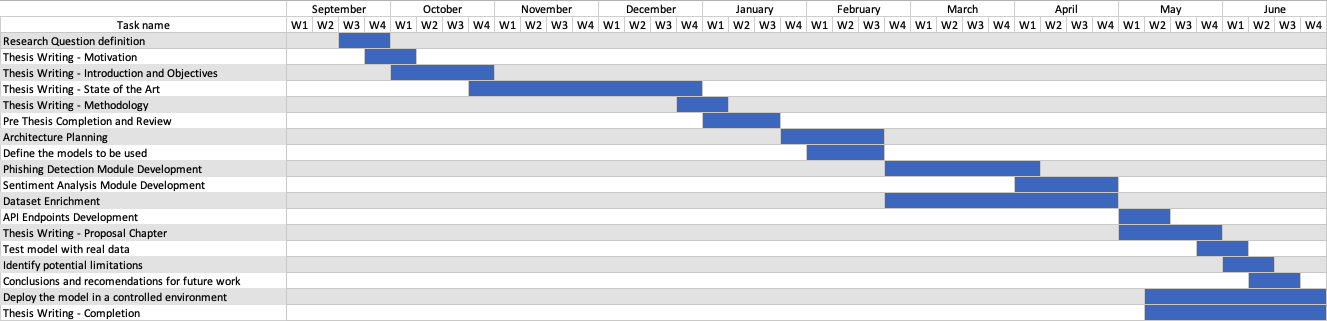
\includegraphics[width=23cm, angle=90]{figs/gantt_chart.png}
        \caption{Gantt diagram containing the tasks that will be developed during this thesis work.}
        \label{fig:c3:gantt_chart}
    \end{center}
  \end{figure}